\documentclass{beamer}
% Class options include: notes, handout, trans
%                        
\usepackage[finnish]{babel}
% Theme for beamer presentation.
\usepackage{beamerthemesplit} 
% Other themes include: beamerthemebars, beamerthemelined,beamerthemetree, beamerthemeplain
\usepackage[utf8]{inputenc}
\usefonttheme{professionalfonts}

\title[Aalto-yliopiston perustieteiden korkeakoulu]{Kysyntäohjautuvan joukkoliikenteen matemaattisia malleja ja algoritmeja}
%\subtitle{Examples of lists, columns and graphics}    % Enter your title between curly braces
\author[L. Häme]{Lauri Häme}                 % Enter your name between curly braces
\institute[Aalto-yliopiston perustieteiden korkeakoulu]{Aalto-yliopiston perustieteiden korkeakoulu}      % Enter your institute name between curly braces
\date{\today}      % Enter the date or \today between curly braces

\usepackage{graphicx}

\begin{document}

% Creates title page of slide show using above information
\begin{frame}
  \titlepage
\end{frame}
%\note{Talk for 30 minutes} % Add notes to yourself that will be displayed when typeset with the notes class option.

\section{Johdanto}
% Creates table of contents slide incorporating all \section and \subsection commands.
%\begin{frame}
%  \tableofcontents
%\end{frame}

\subsection{Johdanto}
\begin{frame}
  \frametitle{Johdanto}   % Insert frame title between curly braces
  \begin{itemize}
    \item 
Kysyntäohjautuva joukkoliikenne = bussi- ja taksipalvelujen välimuoto, joka perustuu ajoneuvojen joustavaan reititykseen
\item
Väitöskirjan tärkeimpiä tuloksia ovat älykkäät reitinlaskentamenetelmät
\item
Menetelmiä voidaan joukkoliikenteen lisäksi hyödyntää esim.
rahti- ja lentoliikenteessä, lähetti- ja ruoankuljetuspalveluissa sekä sotilaslogistiikassa
  \end{itemize}
\end{frame}


%\subsection{Problem formulation}
\begin{frame}
  \frametitle{Kysyntä \& tarjonta}   % Insert frame title between curly braces
%  \begin{columns}[c]
%  \column{2.5in}  % slides are 3in high by 5in wide
  \begin{itemize}
\item
Ajoneuvojen reitinlaskenta, ohjauslogiikka
\begin{itemize}
\item
Esim. Kutsuplus
\end{itemize}
\item
Matkustajien matkansuunnitteluongelma
\begin{itemize}
\item
Esim. Reittiopas
\end{itemize}
\item
Taloudellinen tasapaino
\end{itemize}
%  \column{2.5in}


%\framebox{\includegraphics[scale=0.6]{esitys01}}
 
%  \end{columns}
\end{frame}

\section{Reitinlaskenta}
\subsection{Ongelman määrittely}
\begin{frame}
  \frametitle{Kauppamatkustajan ongelma}   % Insert frame title between curly braces
  \begin{itemize}
    \item 
Tunnetuin reitinlaskentaongelma on ns. kauppamatkustajan ongelma (Traveling Salesman Problem, TSP)
\begin{itemize}
\item
Joukko maantieteellisiä pisteitä, joiden väliset etäisyydet tunnetaan
\item
Tavoitteena on löytää lyhin reitti joka kulkee kaikkien pisteiden kautta
\item
Laskennallisesti haastava ongelma
    \end{itemize}
    \end{itemize}
    \end{frame}

    
    \begin{frame}
  \frametitle{Kauppamatkustajan ongelma, esimerkki}   % Insert frame title between curly braces
\centering
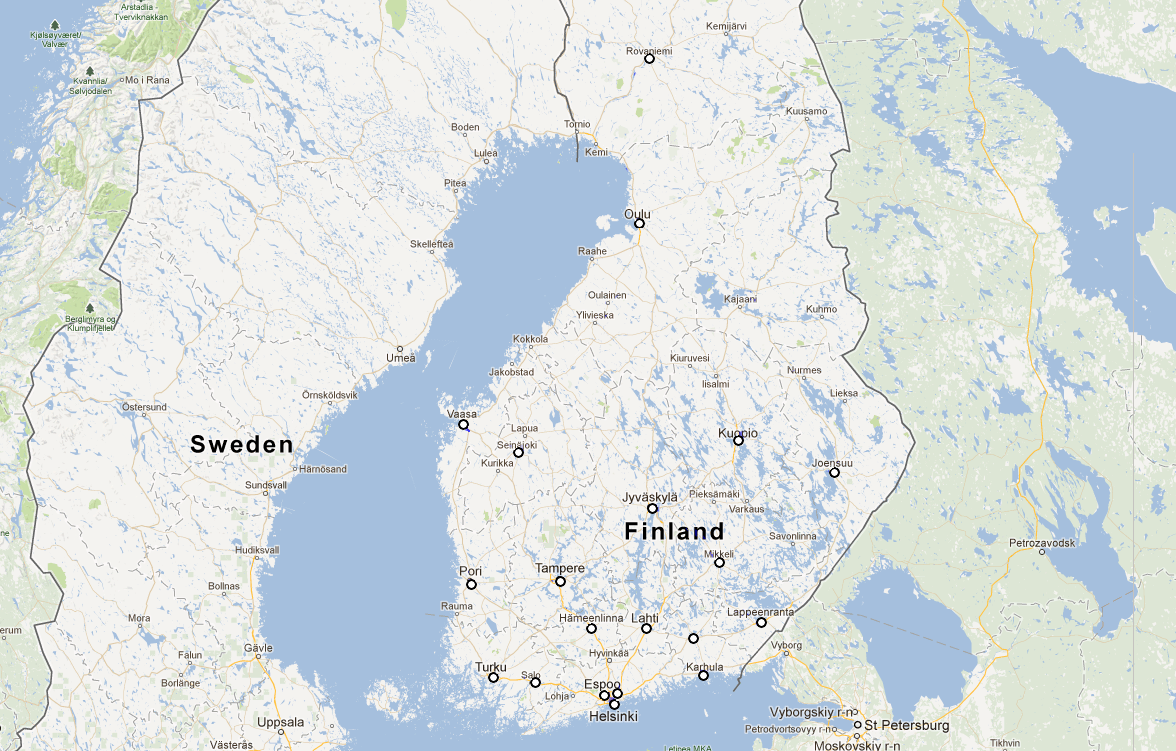
\includegraphics[scale=0.25]{tspdemo01}
    \end{frame}
    
        \begin{frame}
  \frametitle{Kauppamatkustajan ongelma, esimerkki}   % Insert frame title between curly braces
\centering
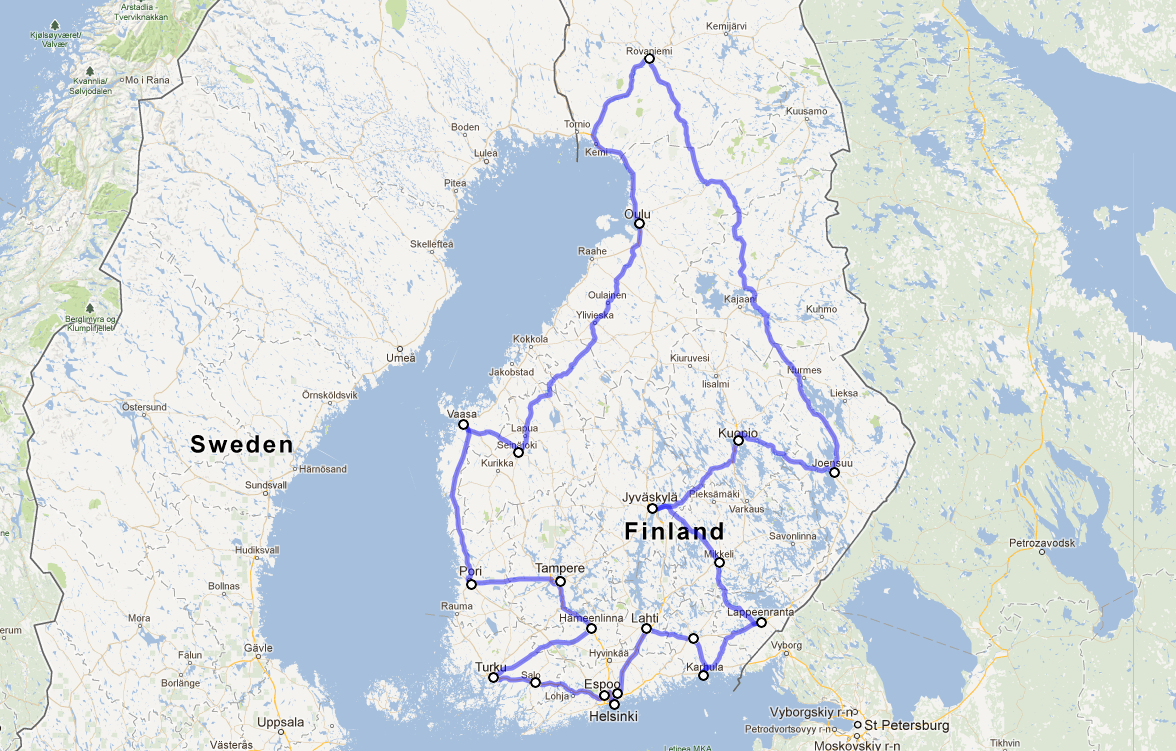
\includegraphics[scale=0.25]{tspdemo02}
    \end{frame}
    

%\subsection{Kysyntäohjautuva joukkoliikenne}
\begin{frame}
    \frametitle{Reitinlaskenta kuljetuspalveluissa}
    \begin{itemize}
    \item
    Käytännössä, esim. kuljetuspalveluissa, reitinlaskentaongelma on usein monimutkaisempi
    \item
    Rajoituksia
    \begin{itemize}
\item 
Kapasiteetti - Ajoneuvoihin mahtuu vain tietty määrä tavaraa/ matkustajia kerrallaan
\item
Aika - Kuljetus ei saa kestää liian kauan
\item
Edeltävyys - Esim. noutopisteessä pitää käydä ennen toimituspistettä
\end{itemize}
\item
Tavoitefunktio: Lyhin reitti ei välttämättä ole paras
\item
Ajoneuvoja eli laskettavia reittejä voi olla useita
  \end{itemize}

\end{frame}




\begin{frame}
  \frametitle{Reitinlaskenta kysyntäohjautuvassa joukkoliikenteessä}   % Insert frame title between curly braces
  \begin{columns}[c]
  \column{3.5in}  % slides are 3in high by 5in wide
  \begin{itemize}
    \item 
    Kysyntäohjautuva joukkoliikenne perustuu pienten tai keskisuurten ajoneuvojen (esim. minibussien) joustavaan reititykseen 
    \item
    Asiakkaat voivat tilata matkoja reaaliaikaisesti esim. internet-käyttöliittymällä
    \item
    Ajoneuvojen reitit muodostuvat tilattujen matkojen perusteella
    \item
    Kunkin matkatilauksen yhteydessä ratkaistaan reitinlaskentaongelma
    %kaksi tehtävää:
    %\begin{itemize}
    %\item
    %Ajoneuvon valinta 
    %\item
    %Valitun ajoneuvon reitin optimointi
    %\end{itemize}
  \end{itemize}
    \column{1.5in}
\centering

%\framebox{
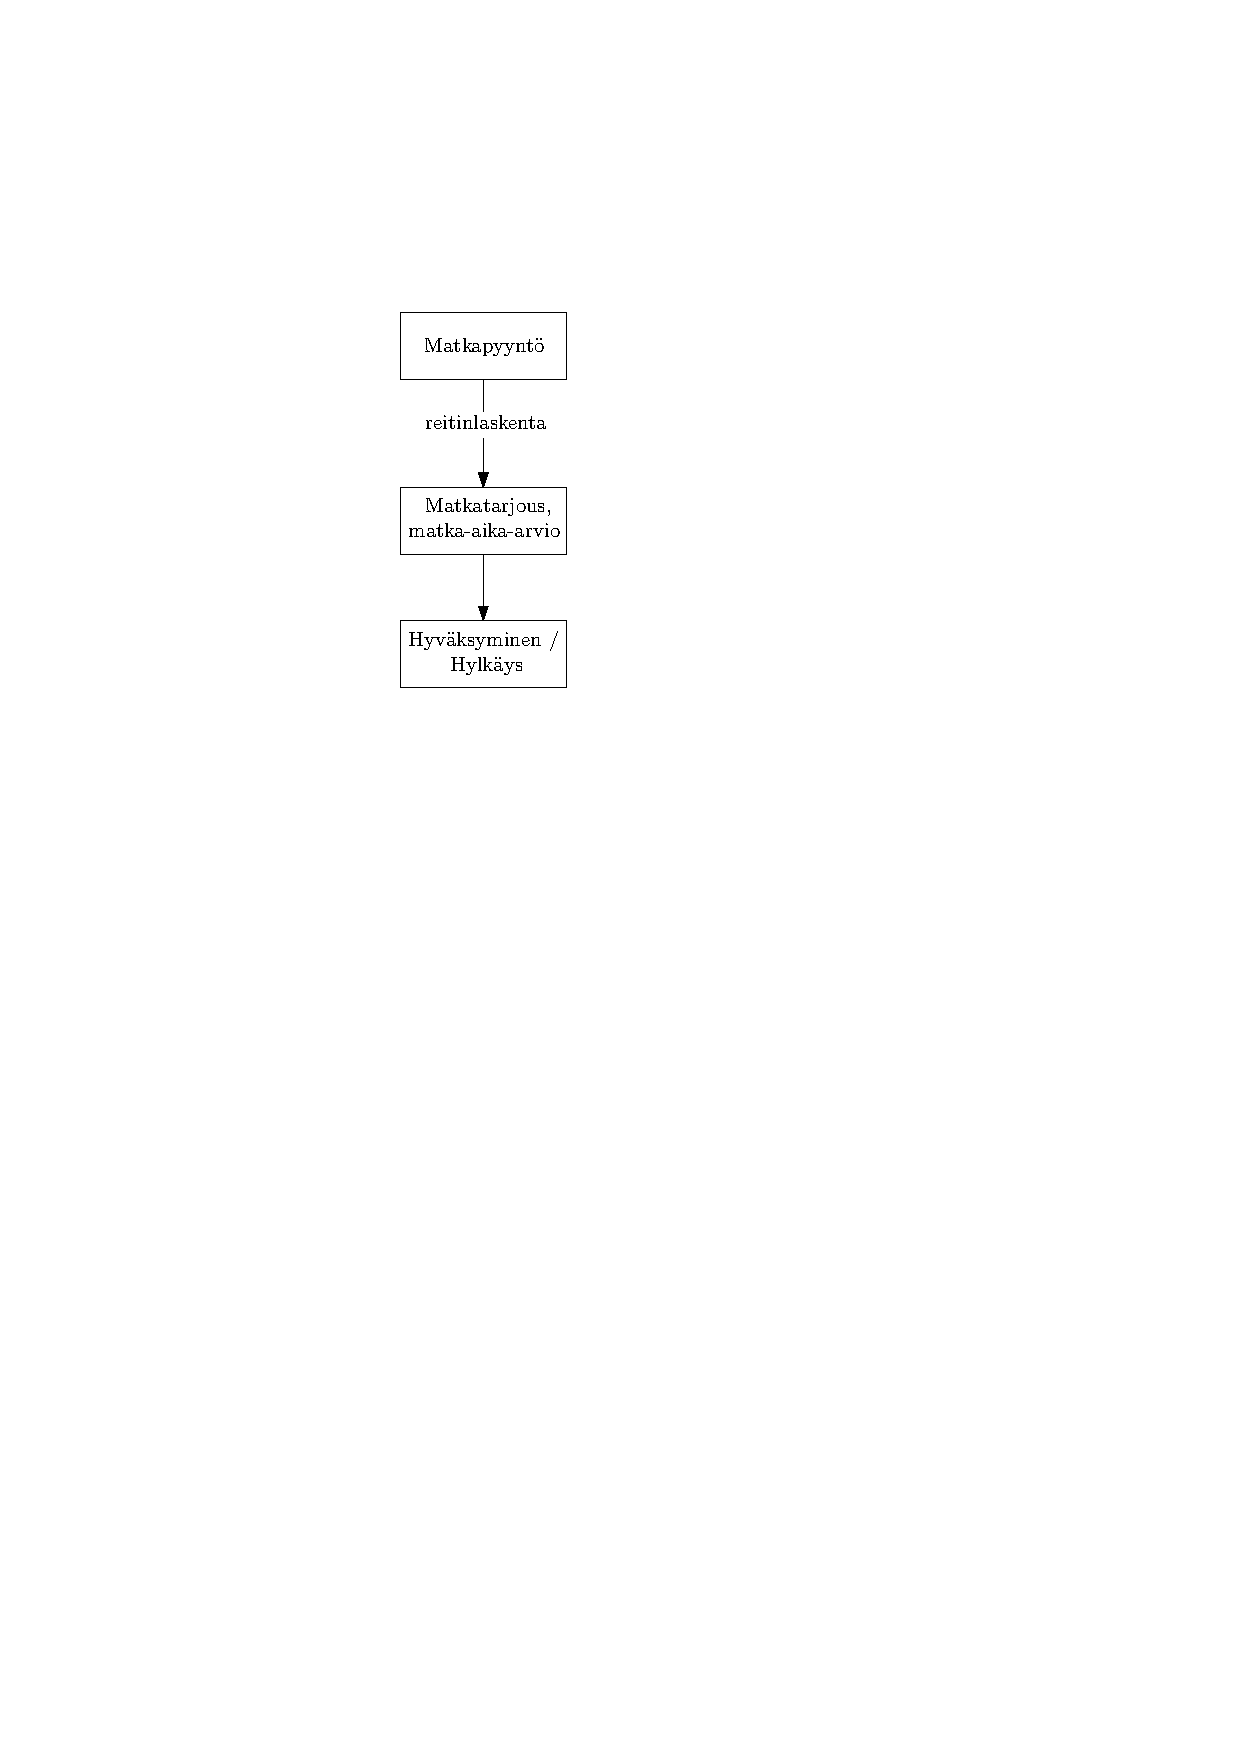
\includegraphics[scale=0.8]{tilauskaavio02}
%}
 
  \end{columns}
\end{frame}

        \begin{frame}
  \frametitle{Kysyntäohjautuva joukkoliikenne, 1 ajoneuvo, esimerkki }   % Insert frame title between curly braces
\begin{center}
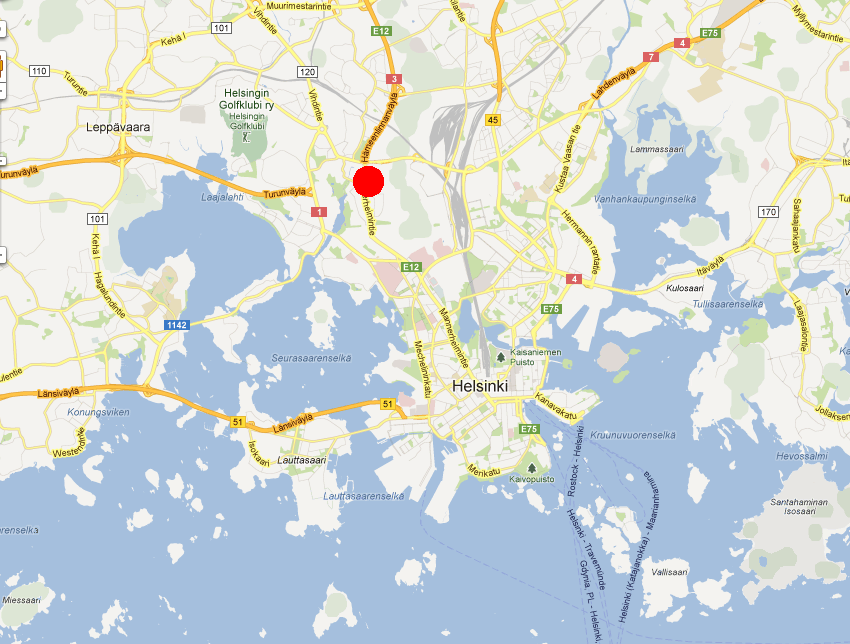
\includegraphics[scale=0.3]{ekademo01}
\end{center}
\end{frame}

        \begin{frame}
  \frametitle{Kysyntäohjautuva joukkoliikenne, 1 ajoneuvo, esimerkki}   % Insert frame title between curly braces
\begin{center}
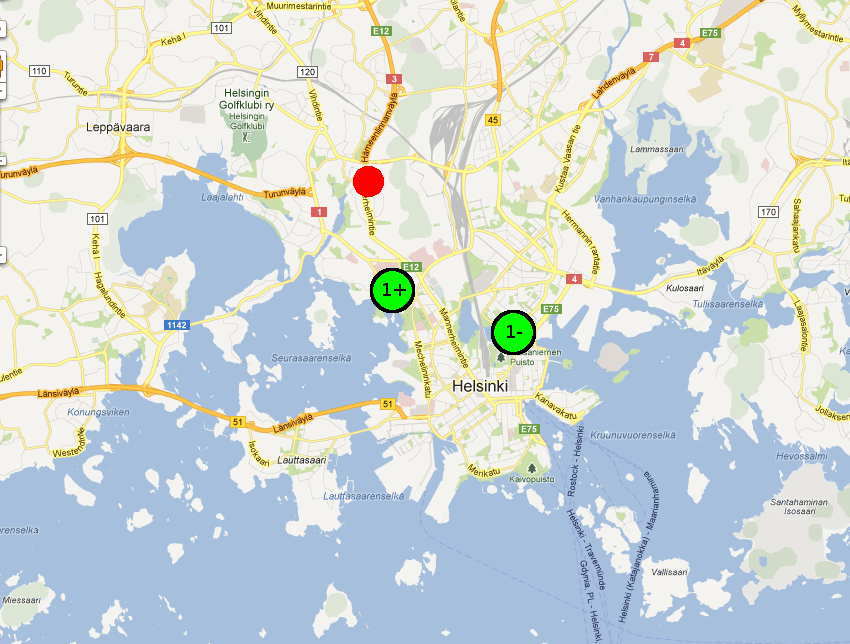
\includegraphics[scale=0.3]{ekademo02}
\end{center}
    \end{frame}
    
            \begin{frame}
  \frametitle{Kysyntäohjautuva joukkoliikenne, 1 ajoneuvo, esimerkki}   % Insert frame title between curly braces
\begin{center}
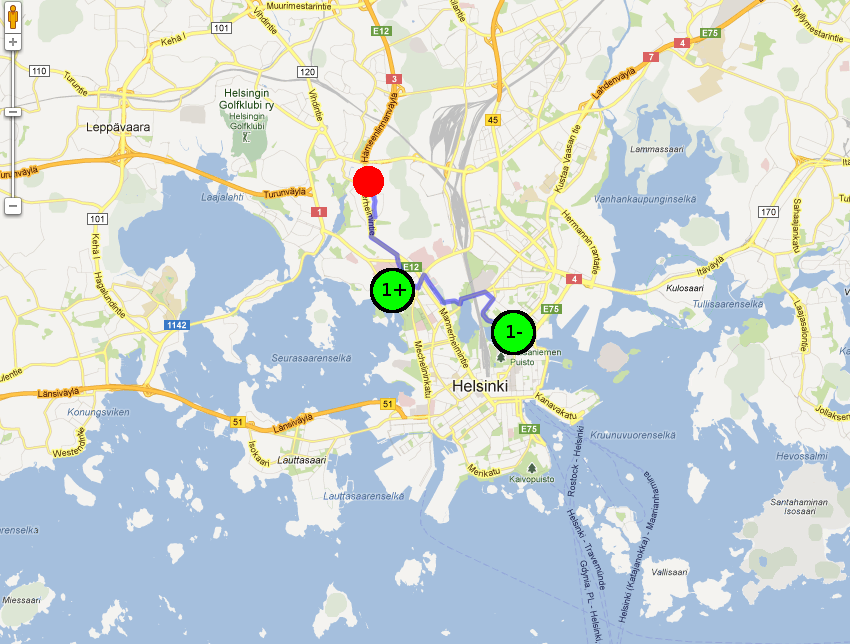
\includegraphics[scale=0.3]{ekademo03}
\end{center}
    \end{frame}
    
            \begin{frame}
  \frametitle{Kysyntäohjautuva joukkoliikenne, 1 ajoneuvo, esimerkki}   % Insert frame title between curly braces
\begin{center}
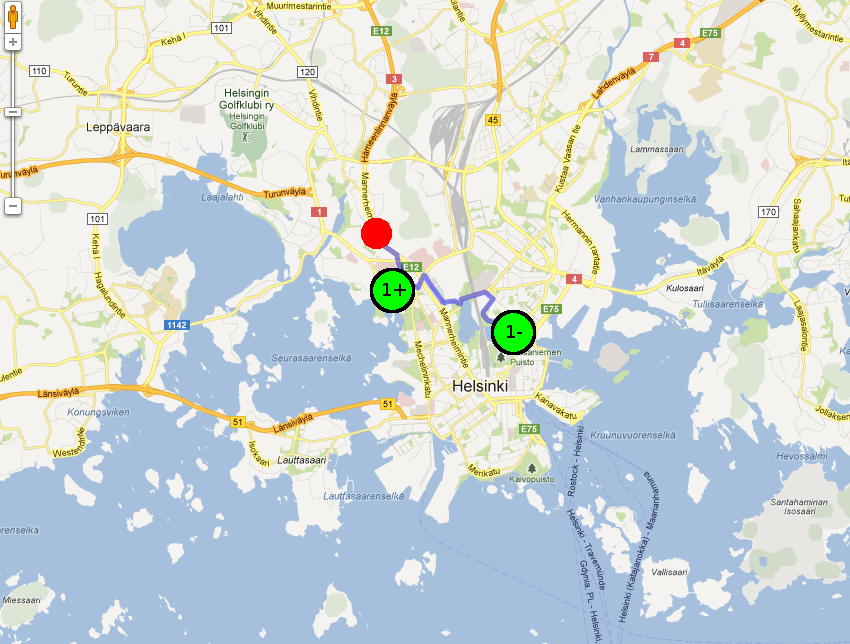
\includegraphics[scale=0.3]{ekademo04}
\end{center}
    \end{frame}
    
            \begin{frame}
  \frametitle{Kysyntäohjautuva joukkoliikenne, 1 ajoneuvo, esimerkki}   % Insert frame title between curly braces
\begin{center}
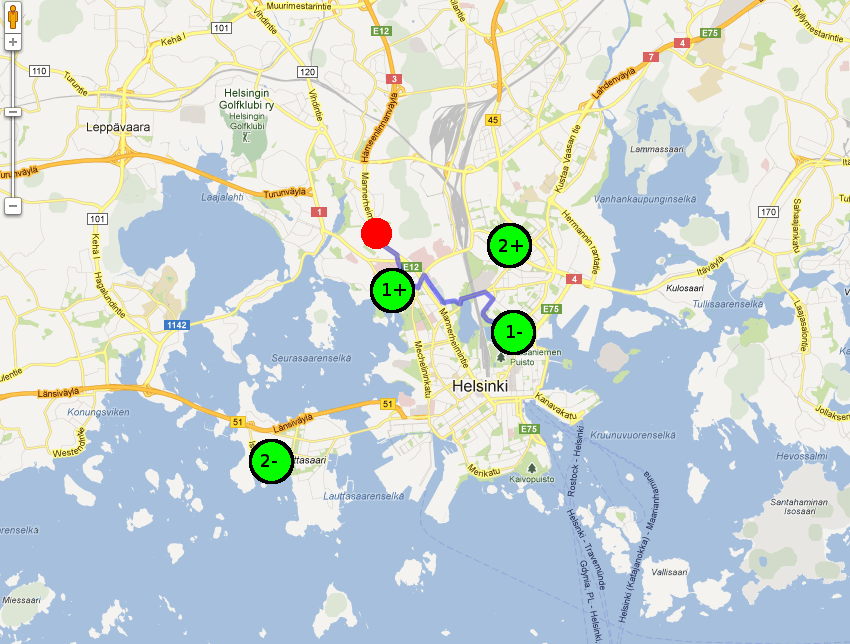
\includegraphics[scale=0.3]{ekademo05}
\end{center}
    \end{frame}
    
            \begin{frame}
  \frametitle{Kysyntäohjautuva joukkoliikenne, 1 ajoneuvo, esimerkki}   % Insert frame title between curly braces
\begin{center}
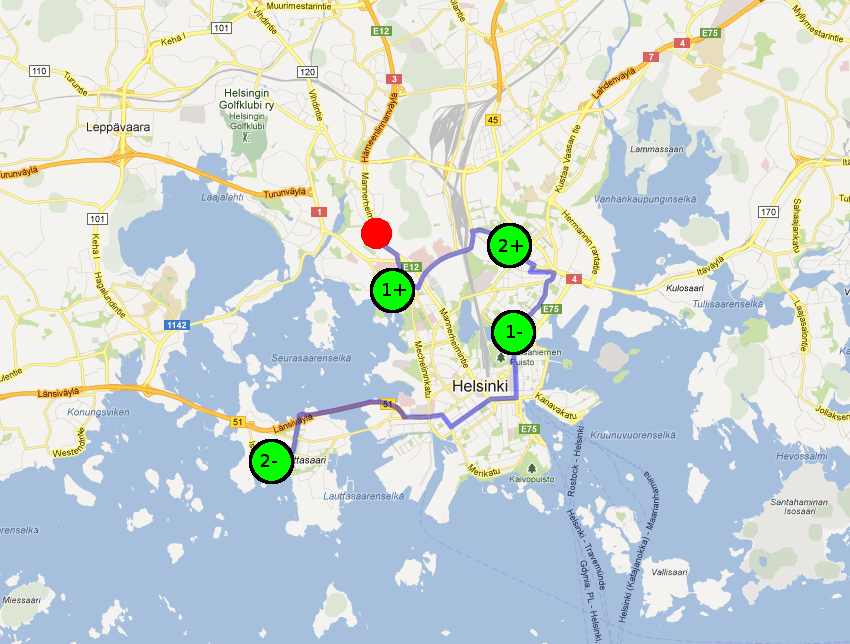
\includegraphics[scale=0.3]{ekademo06}
\end{center}
    \end{frame}

    
\begin{frame}
\frametitle{Aikaikkunat}
\begin{itemize}
 \item 
 Matka-aika voi pidentyä yllättäen reittimuutosten johdosta
 \item
 Palvelutasosta voidaan huolehtia ns. \emph{aikaikkunoilla}
 \begin{itemize}
  \item 
  Esim. lähtö aikaisintaan klo 12:00, perillä viimeistään klo 13:00.
  \item 
  Aikaikkunat voivat olla osittain asiakkaan ja osittain järjestelmän määrittämiä
 \end{itemize}
 \item
 Aikaikkunoita käytetään reitinlaskennassa, jotta tietty minimipalvelutaso toteutuisi
 \item
 Liian tiukat aikaikkunat vähentävät reitin joustavuutta
\end{itemize}
\begin{center}
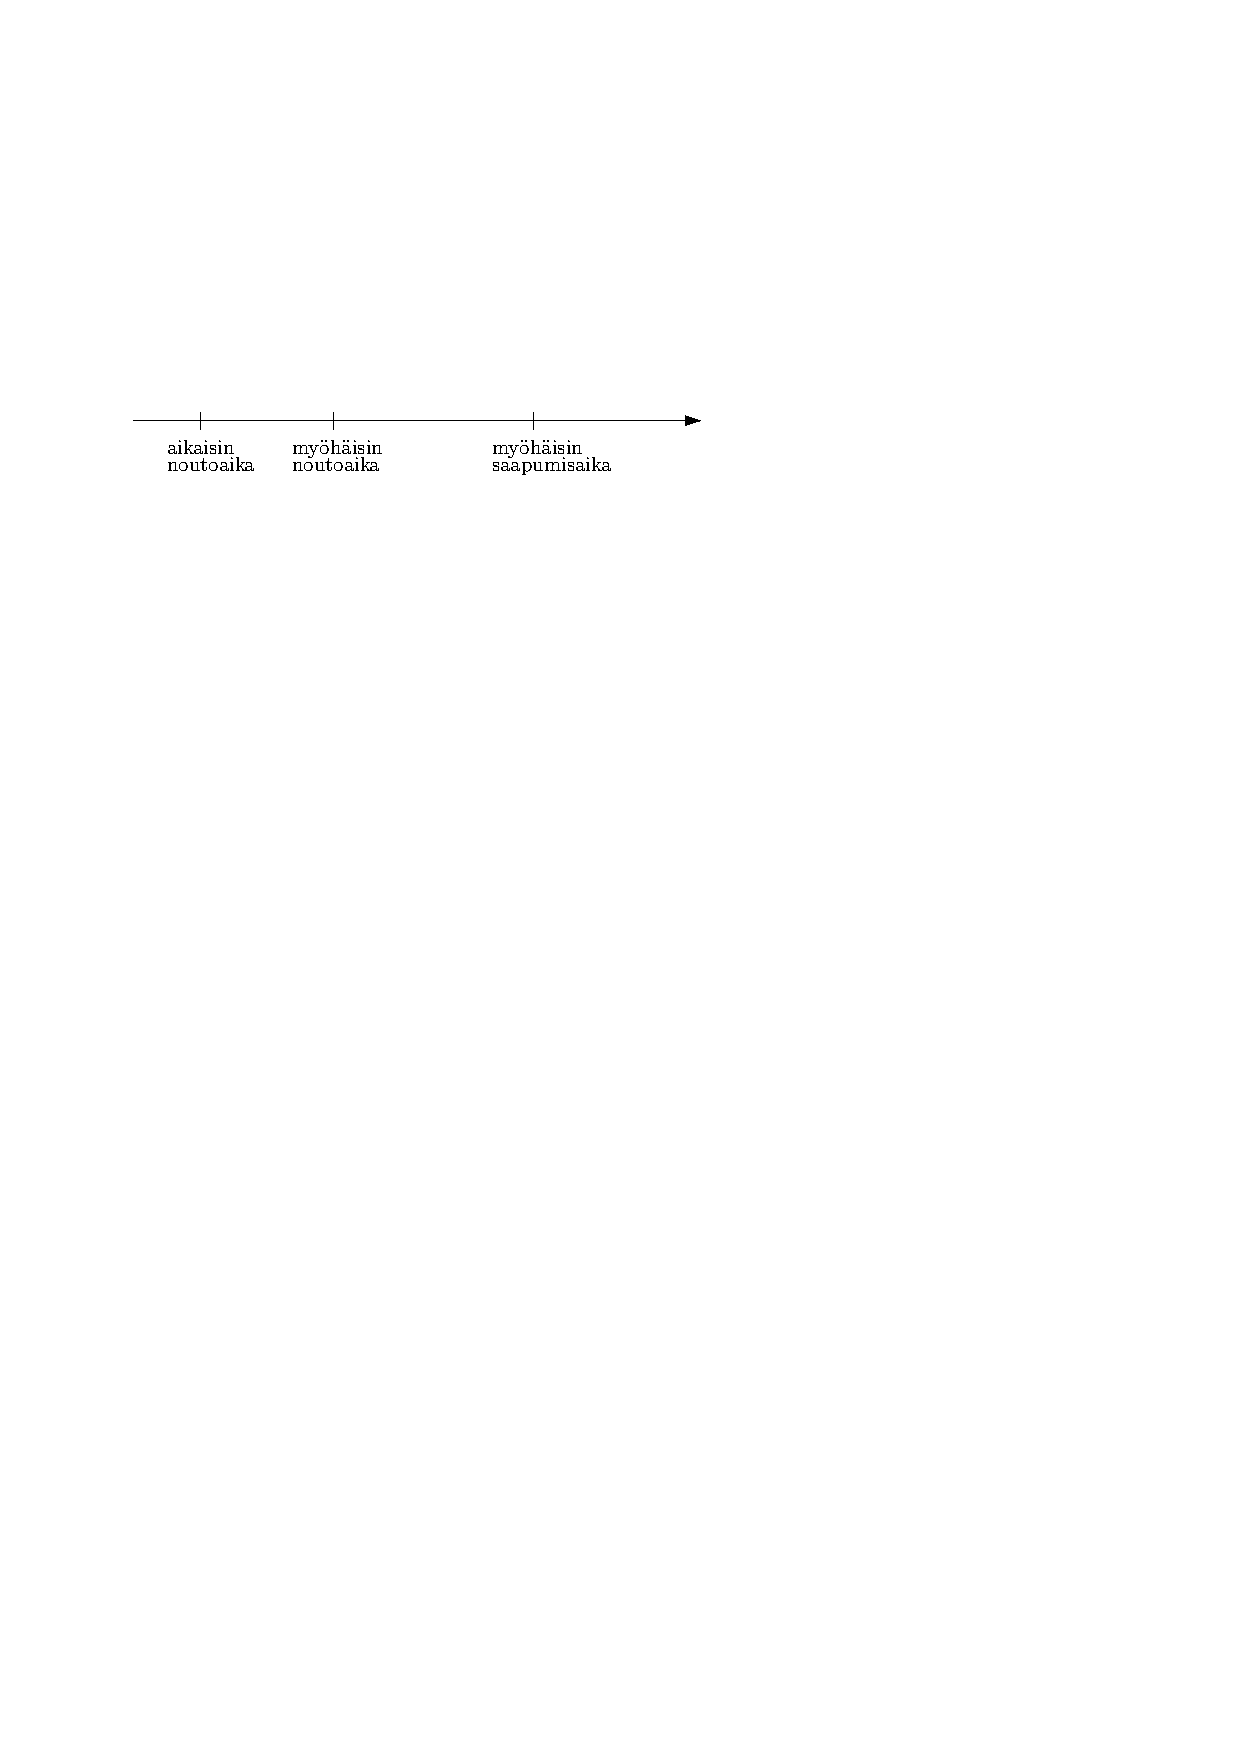
\includegraphics[scale=0.8]{aikaikkuna01}
\end{center}
\end{frame}    
    
    
    
\begin{frame}
  \frametitle{Ajoneuvon ja reitin valintaongelma}   % Insert frame title between curly braces
\begin{itemize}
 \item 
 Usean ajoneuvon tapauksessa jokaiselle uudelle asiakkaalle valitaan ajoneuvo ja valitulle ajoneuvolle määrätään uusi reitti
  \item
 Ajoneuvon ja reitin valinnassa pitää ottaa huomioon mm.
 \begin{itemize}
  \item 
  Uuden asiakkaan aiheuttama reitin pitenemä
  \item
  Uuden asiakkaan palvelutaso ja muille asiakkaille aiheutuva palvelutason muutos
  \item
  Kysyntäennuste
 \end{itemize}
%\end{itemize}
%\begin{center}
% 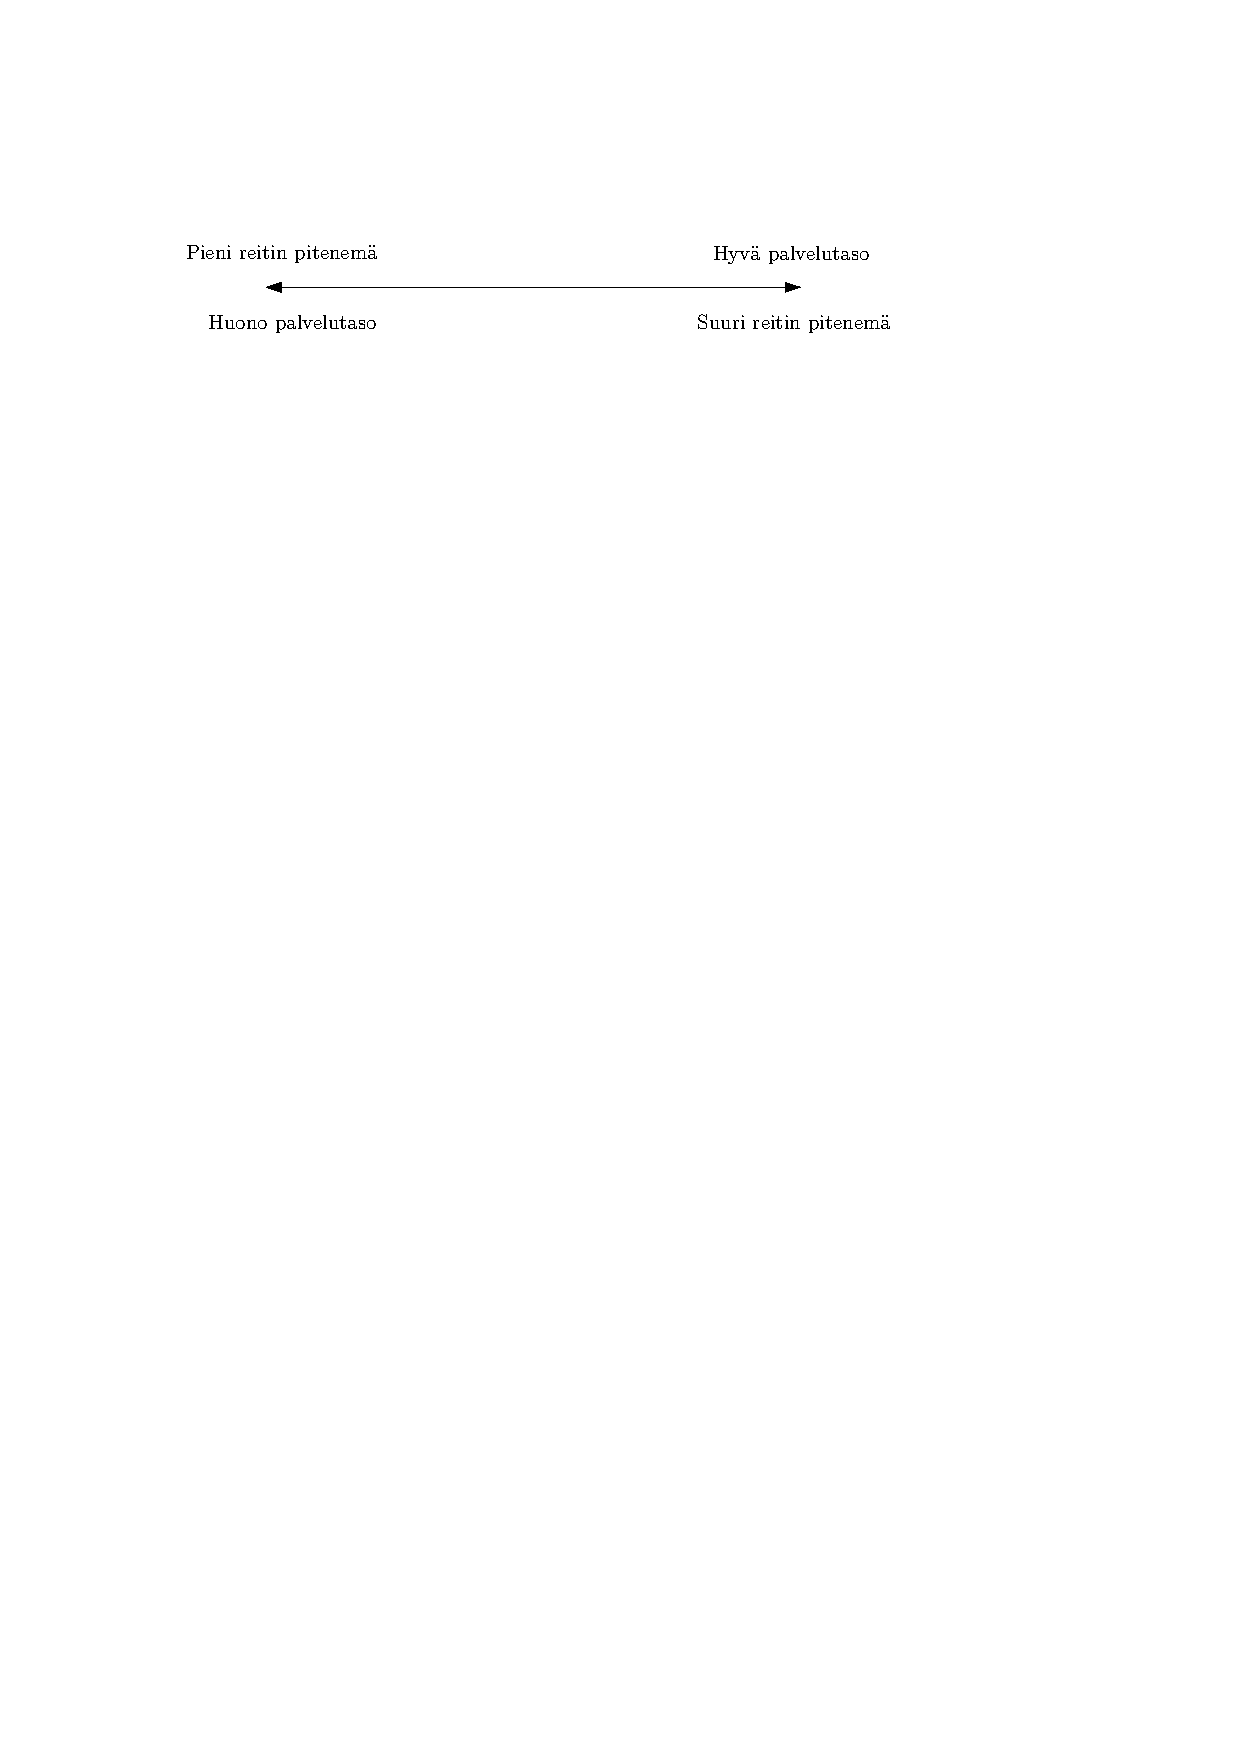
\includegraphics[scale=0.6]{vskuvatavoite}
%\end{center}
\item
Yleisesti jos minimoidaan reitin pituutta, palvelutaso saattaa kärsiä ja jos optimoidaan ainoastaan palvelutasoa, kustannukset kasvavat
%\begin{itemize}
\end{itemize}
\end{frame}

\subsection{Hajautettu ratkaisu}
\begin{frame}
  \frametitle{Hajautettu ratkaisu}   % Insert frame title between curly braces
\begin{itemize}
\item
Yritetään lisätä uusi asiakas johonkin olemassaolevista reiteistä %$\to$ käsitellään jokainen ajoneuvo erikseen
%\item
%Valitaan se ajoneuvo, jonka reitille uusi asiakas sopii parhaiten
\item
Lasketaan jokaiselle ajoneuvolle uusi reittiehdotus ja valitaan niistä paras/parhaat
\item
Ajoneuvojen reittiehdotukset lasketaan erikseen
\end{itemize}
\end{frame}



                \begin{frame}
  \frametitle{Hajautettu ratkaisu, esimerkki}   % Insert frame title between curly braces
\begin{minipage}[t][0.3\textheight][t]{\textwidth}
  \begin{itemize}
 \item 
 Kaksi ajoneuvoa, joista toinen odottaa tyhjänä
\end{itemize}
  \end{minipage}
  \vfill
  \begin{minipage}{\textwidth}
    \centering
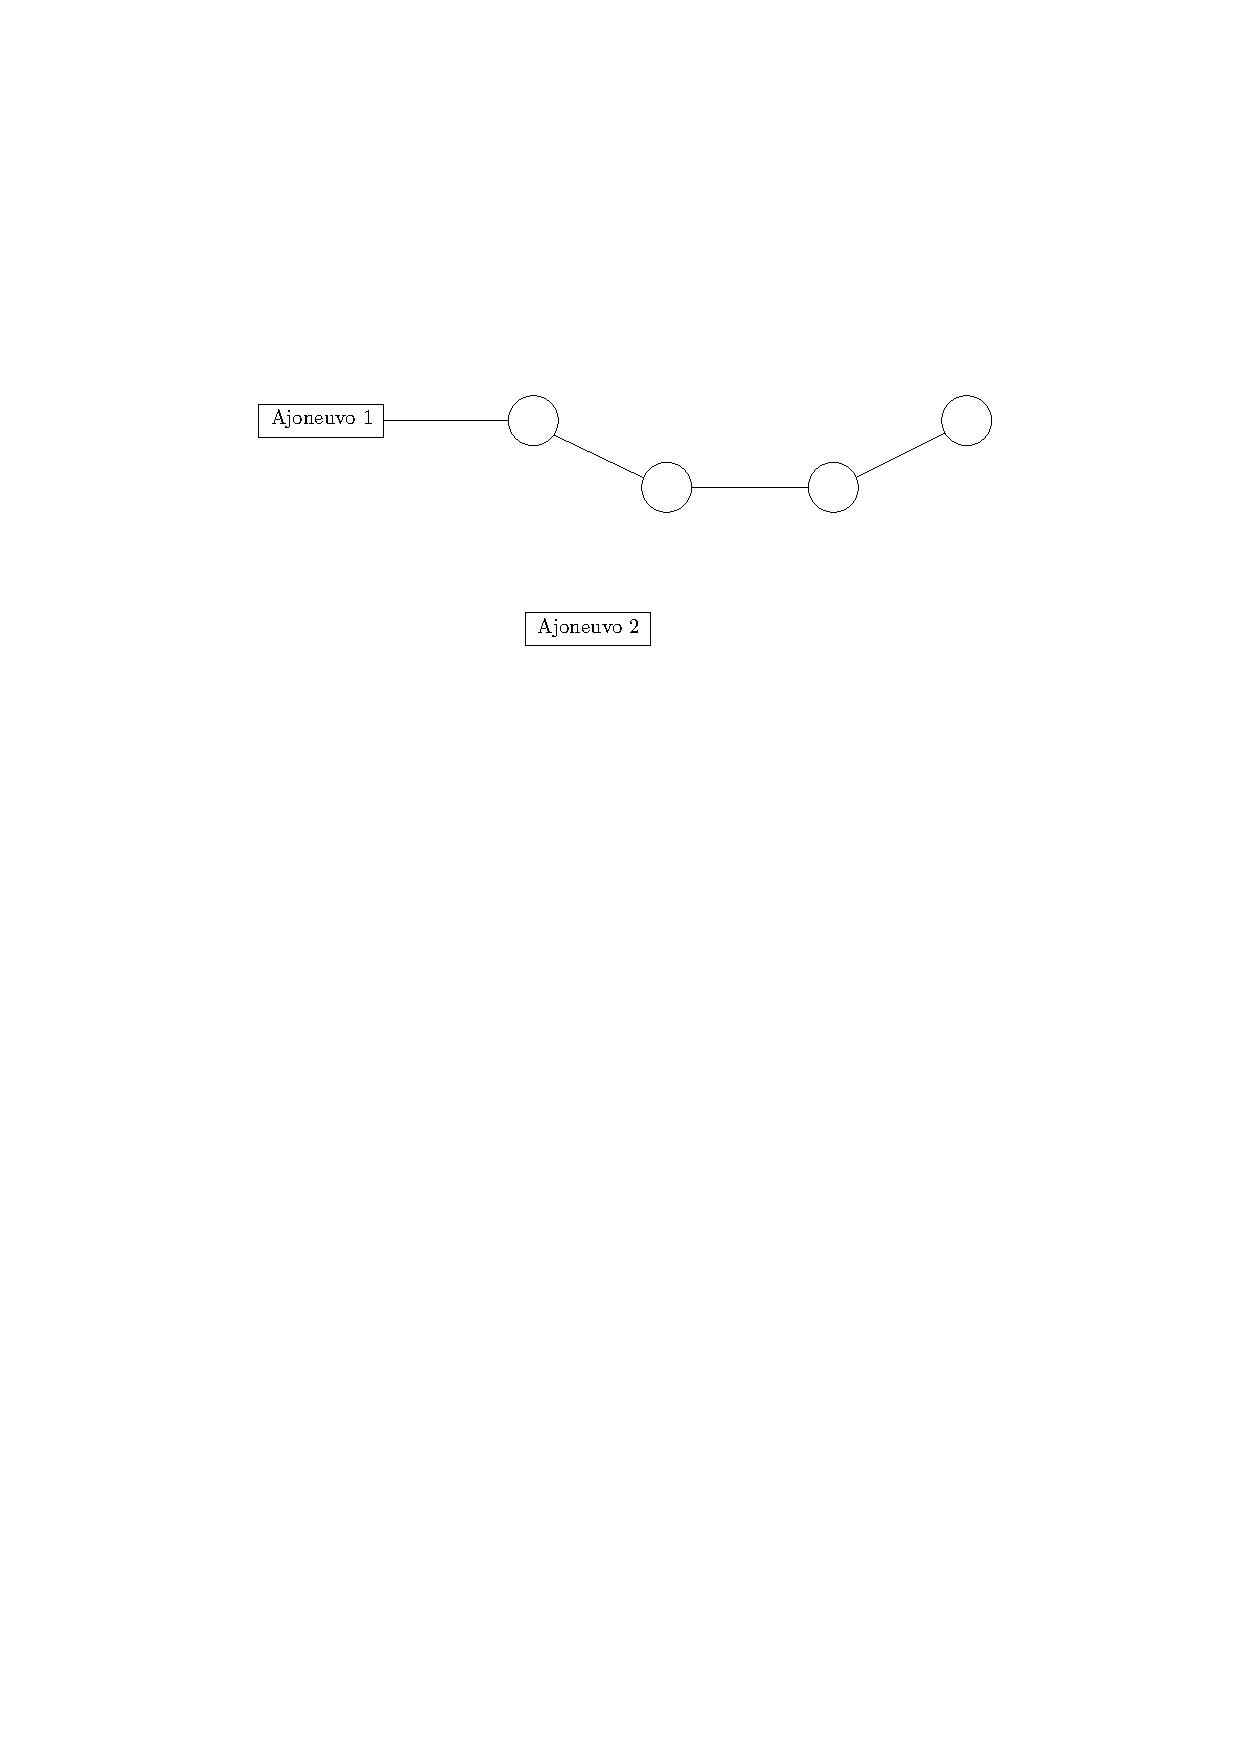
\includegraphics[scale=0.6]{valinta01}
  \end{minipage}
    \end{frame}
    
    
                    \begin{frame}
  \frametitle{Hajautettu ratkaisu, esimerkki}   % Insert frame title between curly braces
\begin{minipage}[t][0.3\textheight][t]{\textwidth}
  \begin{itemize}
 \item 
 Kaksi ajoneuvoa, joista toinen odottaa tyhjänä
   \item 
 Uusi asiakas tilaa matkan ($u^+,u^-$)
\end{itemize}
  \end{minipage}
  \vfill
  \begin{minipage}{\textwidth}
    \centering
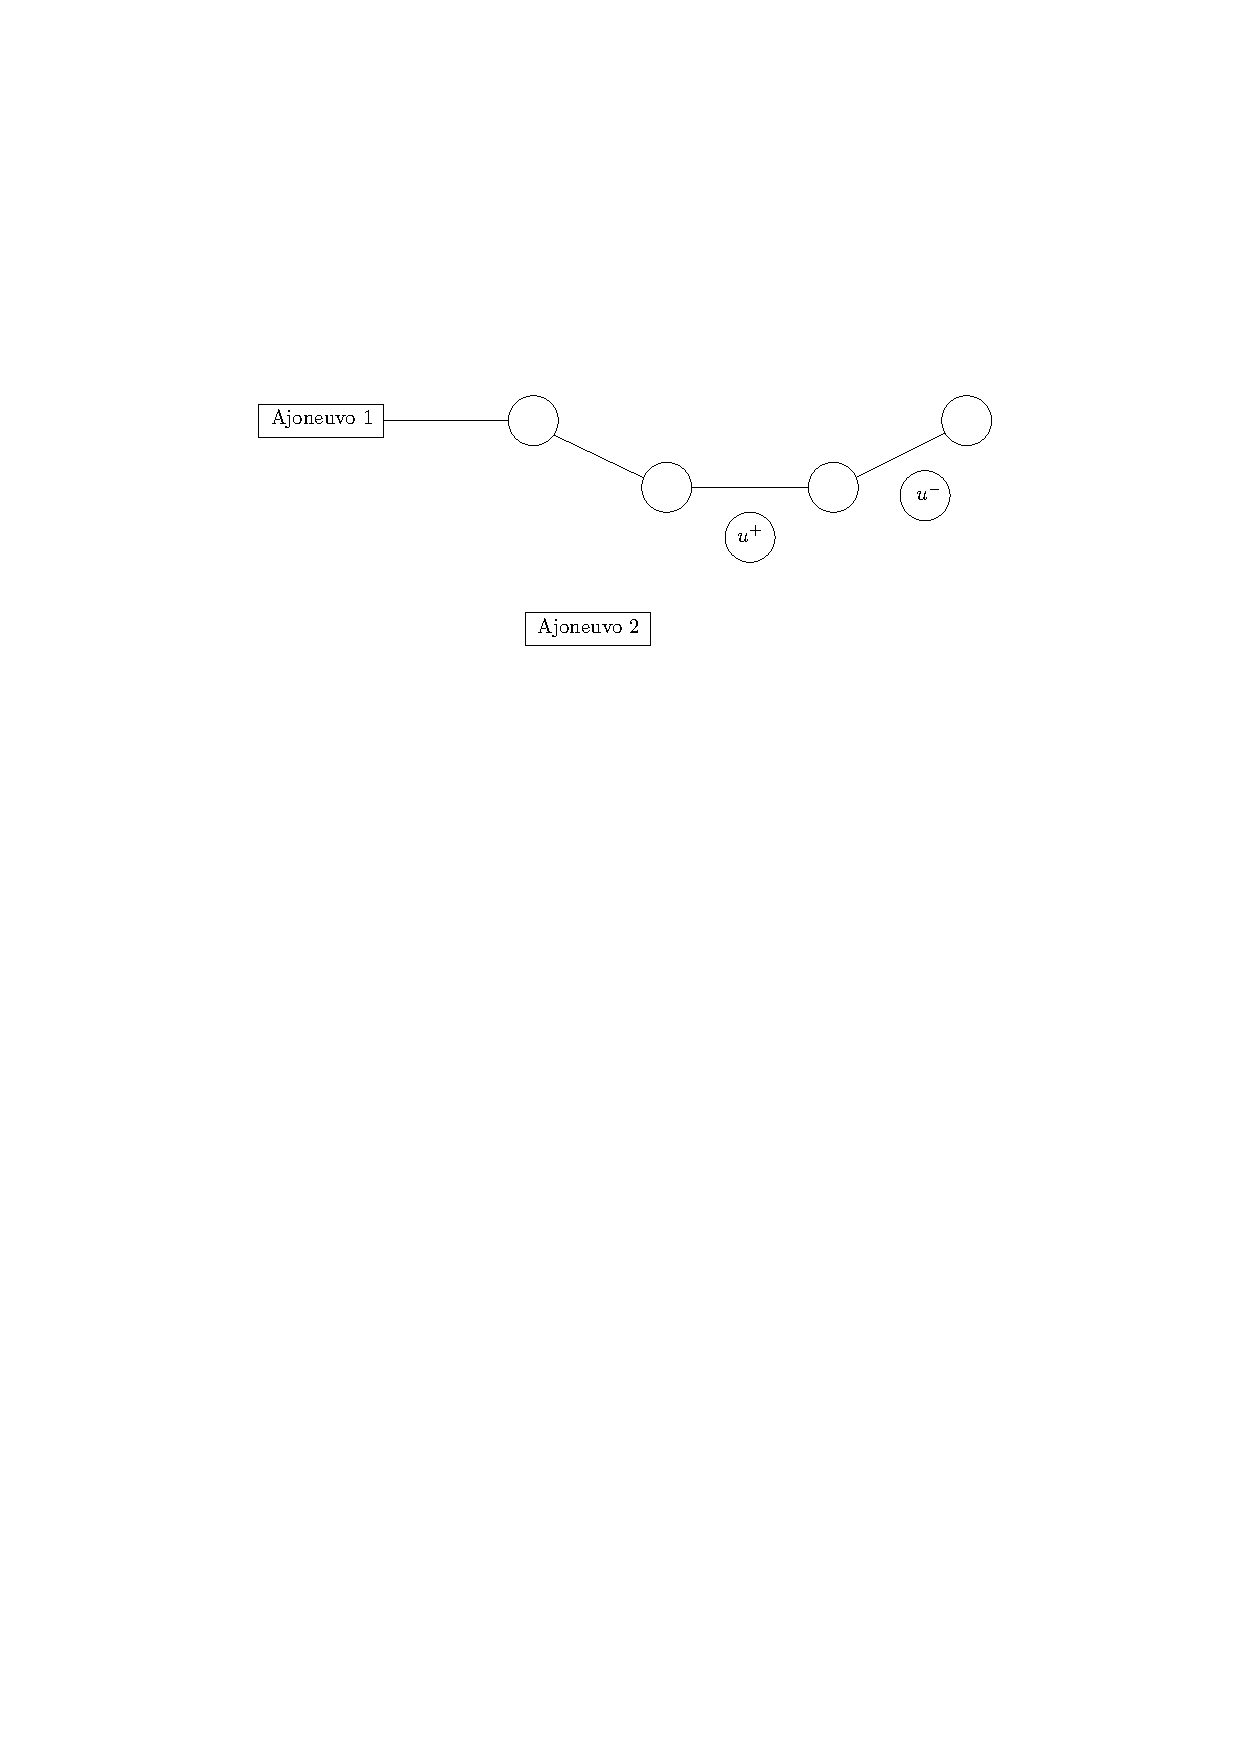
\includegraphics[scale=0.6]{valinta02}
  \end{minipage}
  
  \end{frame}
    
                        \begin{frame}
  \frametitle{Hajautettu ratkaisu, esimerkki}   % Insert frame title between curly braces
\begin{minipage}[t][0.3\textheight][t]{\textwidth}
  \begin{itemize}
 \item 
 Kaksi ajoneuvoa, joista toinen odottaa tyhjänä
   \item 
 Uusi asiakas tilaa matkan ($u^+,u^-$)
 \item
 Ehdotus 1: reitin pitenemä minimoituu, palvelutaso kärsii
\end{itemize}
  \end{minipage}
  \vfill
  \begin{minipage}{\textwidth}
    \centering
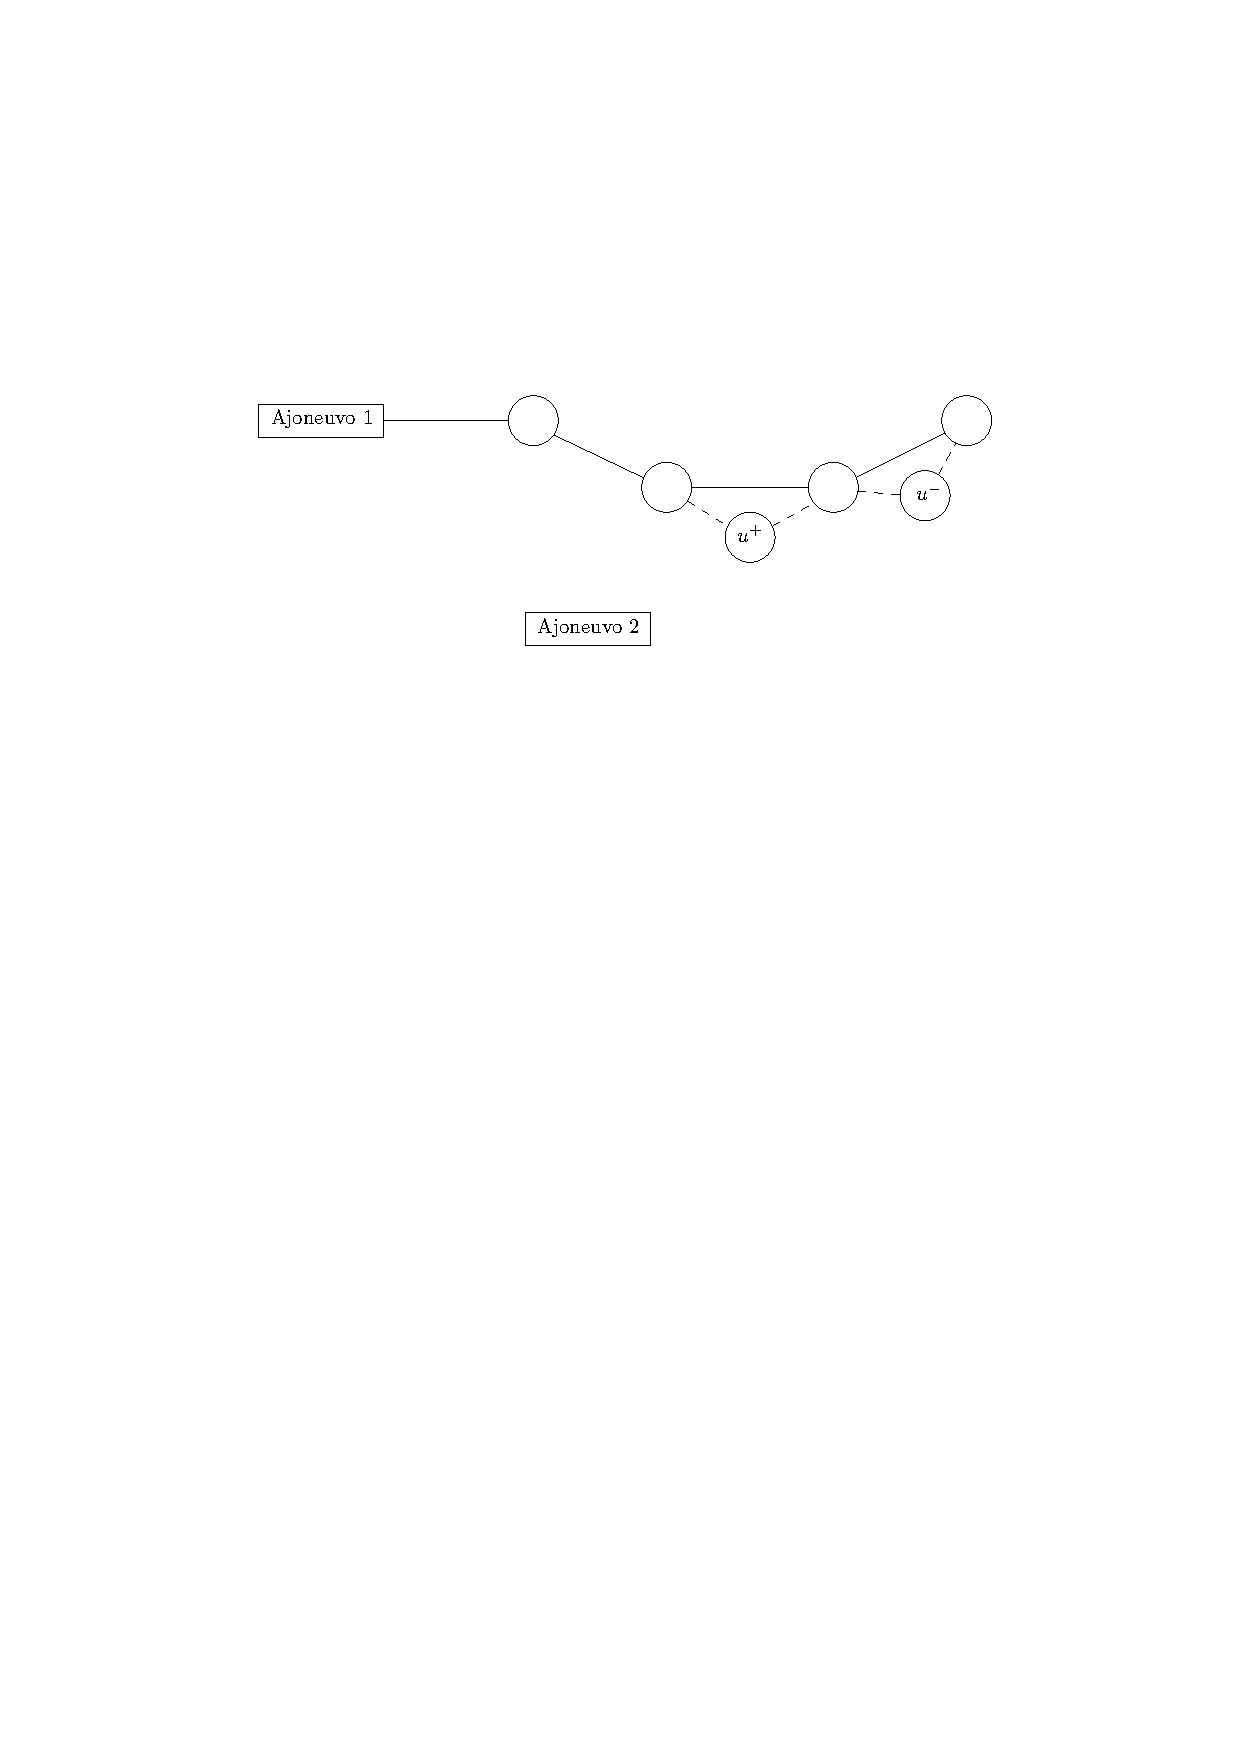
\includegraphics[scale=0.6]{valinta03}
  \end{minipage}
  
  \end{frame}
  
  
                          \begin{frame}
  \frametitle{Hajautettu ratkaisu, esimerkki}   % Insert frame title between curly braces
\begin{minipage}[t][0.3\textheight][t]{\textwidth}
  \begin{itemize}
 \item 
 Kaksi ajoneuvoa, joista toinen odottaa tyhjänä
   \item 
 Uusi asiakas tilaa matkan ($u^+,u^-$)
 \item
 Ehdotus 1: reitin pitenemä minimoituu, palvelutaso kärsii
  \item
 Ehdotus 2: palvelutaso on paras mahdollinen, reitin pituus kasvaa enemmän
\end{itemize}
  \end{minipage}
  \vfill
  \begin{minipage}{\textwidth}
    \centering
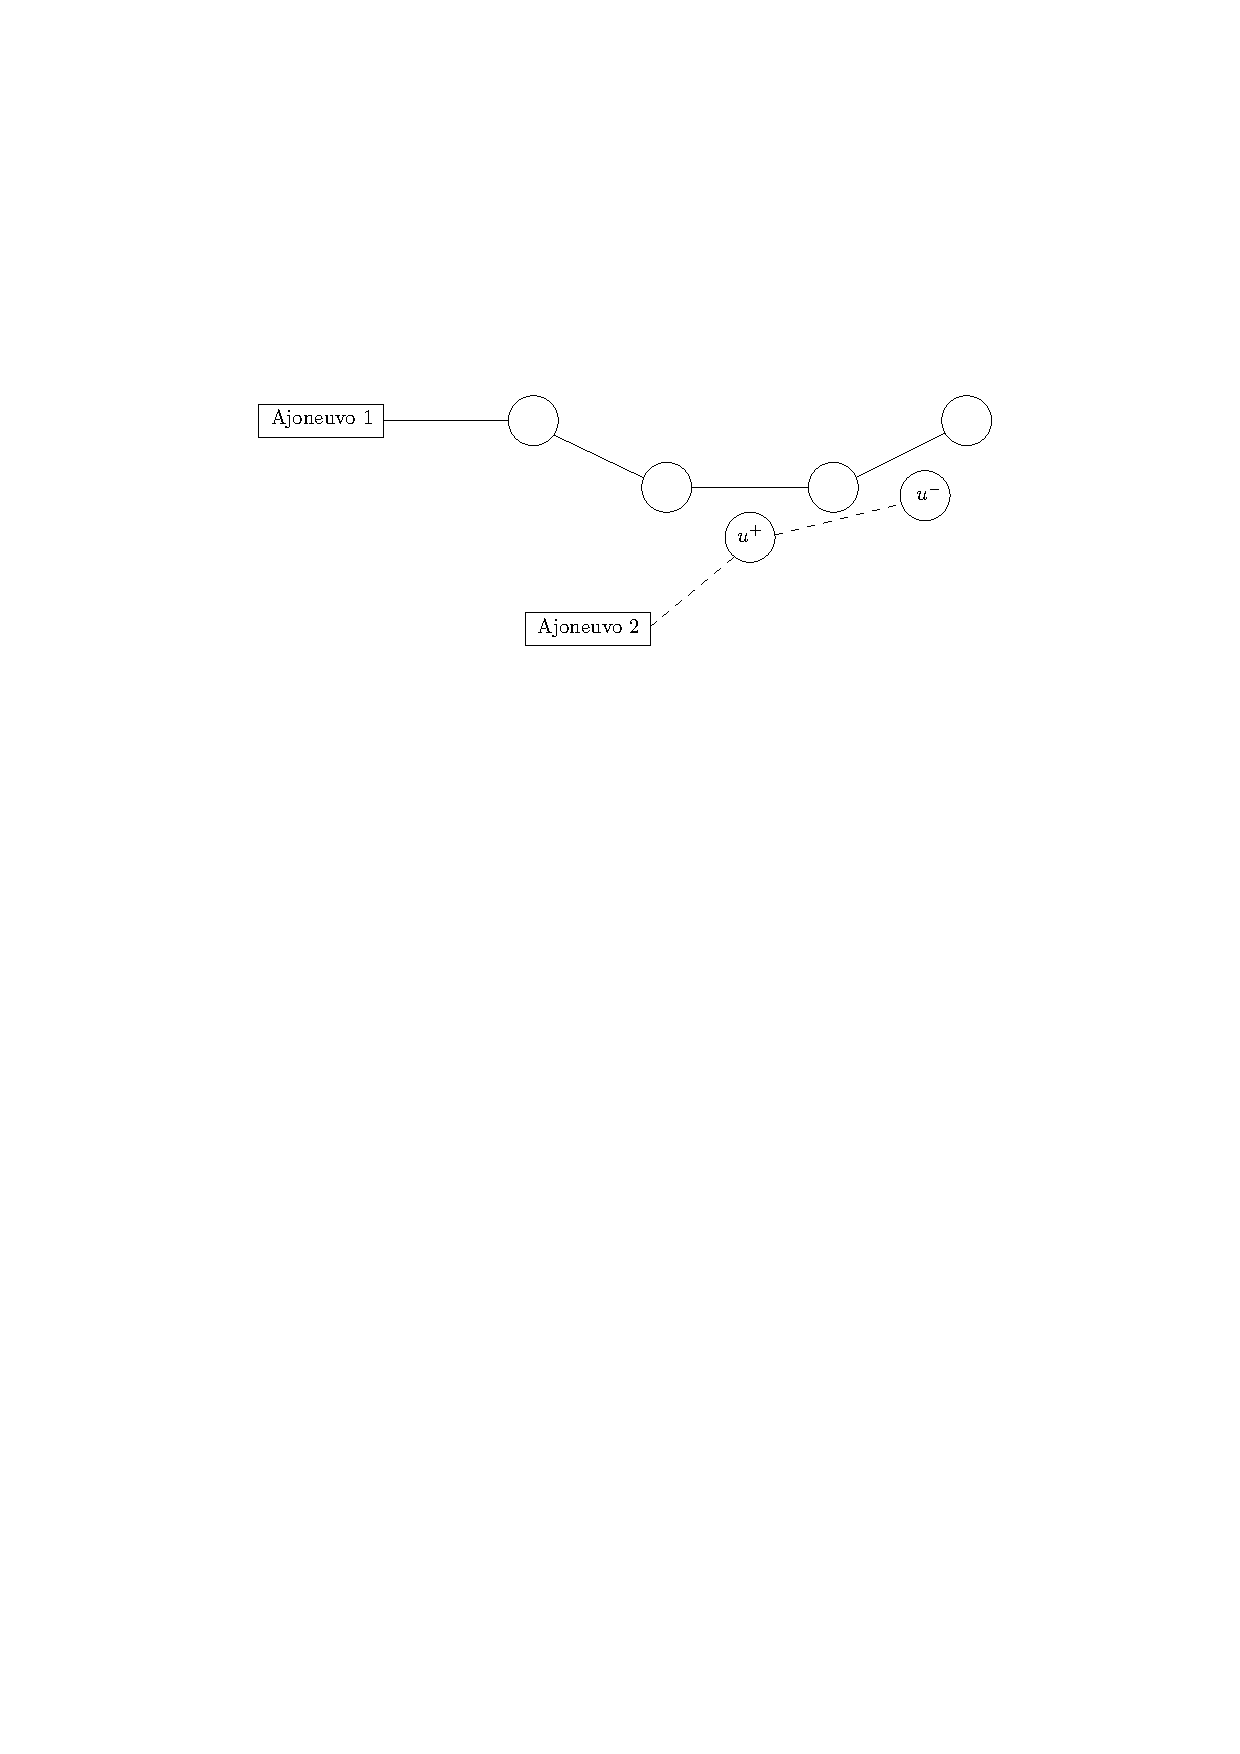
\includegraphics[scale=0.6]{valinta04}
  \end{minipage}
  
  \end{frame}
    

    \begin{frame}
\frametitle{Yksinkertainen lisäysalgoritmi (Insertion algorithm)}
 \begin{itemize}
\item
Yksinkertainen ratkaisu reittiehdotusten laskemiselle on lisätä uuden asiakkaan nouto- ja toimituspiste sopivaan väliin 
\item
Ei-täydellinen ratkaisu: olemassaolevien pisteiden järjestys säilyy
\end{itemize}
\begin{center}
 \includegraphics[scale=0.5]<1>{insertion02}
  \includegraphics[scale=0.5]<2>{insertion03}
   \includegraphics[scale=0.5]<3>{insertion04}
    \includegraphics[scale=0.5]<4>{insertion05}
      \includegraphics[scale=0.5]<5>{insertion06}
       \includegraphics[scale=0.5]<6>{insertion07}
        \includegraphics[scale=0.5]<7>{insertion08}
         \includegraphics[scale=0.5]<8>{insertion09}

           
\end{center}

\end{frame}
    
    \begin{frame}
\frametitle{Laajennettu lisäysalgoritmi (Adaptive insertion algorithm)}
 \begin{itemize}
\item
Rakennetaan lisäysperiaatteella rinnakkain useampi vaihoehtoinen reitti ja valitaan niistä paras
\end{itemize}
\begin{center}
 \includegraphics[scale=0.5]<1>{insertion02}
  \includegraphics[scale=0.5]<2>{insertion03}
   \includegraphics[scale=0.5]<3>{insertion04}
    \includegraphics[scale=0.5]<4>{insertion05}
     \includegraphics[scale=0.5]<5>{insertion06}
      \includegraphics[scale=0.5]<6>{insertion07}
       \includegraphics[scale=0.5]<7>{insertion08}
       \includegraphics[scale=0.5]<8>{insertion09}
\\
\hfill
\\
\hfill
\\
                \includegraphics[scale=0.5]<1>{insertion02}   
                \includegraphics[scale=0.5]<2>{insertion03}
                \includegraphics[scale=0.5]<3>{insertion04}  
                \includegraphics[scale=0.5]<4>{insertion05}
                \includegraphics[scale=0.5]<5>{insertion06b} 
                \includegraphics[scale=0.5]<6>{insertion07b} 
                \includegraphics[scale=0.5]<7>{insertion08b} 
                \includegraphics[scale=0.5]<8>{insertion09b} 
\end{center}

\end{frame}


    \begin{frame}
\frametitle{Täydellinen lisäysalgoritmi (Exact insertion algorithm)}
 \begin{itemize}
 \item
Rakennetaan lisäysperiaatteella rinnakkain kaikki mahdolliset reitit (enintään $\frac{(2n)!}{2^n}$ kpl)
%\item
%Perusidea: luetellaan yhden ajoneuvon kaikki mahdolliset reitit ja valitaan niistä paras 
%\item
%Kaikki mahdolliset reitit ($\frac{(2n)!}{2^n}$ kpl) saadaan lisäämällä asiakkaat yksi kerrallaan \emph{kaikkiin edellisiin} reitteihin
\end{itemize}
\hfill \\
  \begin{columns}[c]
  \column{0.7in}
  \column{2.5in}  % slides are 3in high by 5in wide
 $1^+,1^-$ \\
 \hfill \\
  $1^+,1^-,2^+,2^-$ \\
    $1^+,2^+,1^-,2^-$ \\
     $1^+,2^+,2^-,1^-$ \\
      $2^+,1^+,1^-,2^-$ \\
      $2^+,1^+,2^-,1^-$ \\
      $2^+,2^-,1^+,1^-$ \\
      \column{2.5in}
      {\tiny 
        $1^+,1^-,2^+,2^-,3^+,3^-$ \\
        $1^+,1^-,2^+,3^+,2^-,3^-$ \\
        $1^+,1^-,3^+,2^+,2^-,3^-$ \\
        $1^+,3^+,1^-,2^+,2^-,3^-$ \\
        $3^+,1^+,1^-,2^+,2^-,3^-$ \\
        
        $1^+,1^-,2^+,3^+,3^-,2^-$ \\
        $1^+,1^-,3^+,2^+,3^-,2^-$ \\
        $1^+,3^+,1^-,2^+,3^-,2^-$ \\
        $3^+,1^+,1^-,2^+,3^-,2^-$ \\
        
        $1^+,1^-,3^+,3^-,2^+,2^-$ \\
        $1^+,3^+,1^-,3^-,2^+,2^-$ \\
        $3^+,1^+,1^-,3^-,2^+,2^-$ \\
        
      \ldots
      }
      \end{columns}
\end{frame}
    
        \begin{frame}
\frametitle{Lisäysalgoritmi, tuloksia}
 \begin{itemize}
\item
Tiukkojen aika- tai kapasiteettirajoitusten vallitessa kaikkien mahdollisten reittien lukumäärä pysyy kohtuullisena ja 
täydellinen algoritmi tuottaa nopeasti optimaalisen ratkaisun
\item
Jos rajoitukset eivät ole tiukkoja, saadaan tehokas ratkaisu
rajoittamalla rinnakkaisten reittien lukumäärää
\end{itemize}
\hfill \\
\begin{center}
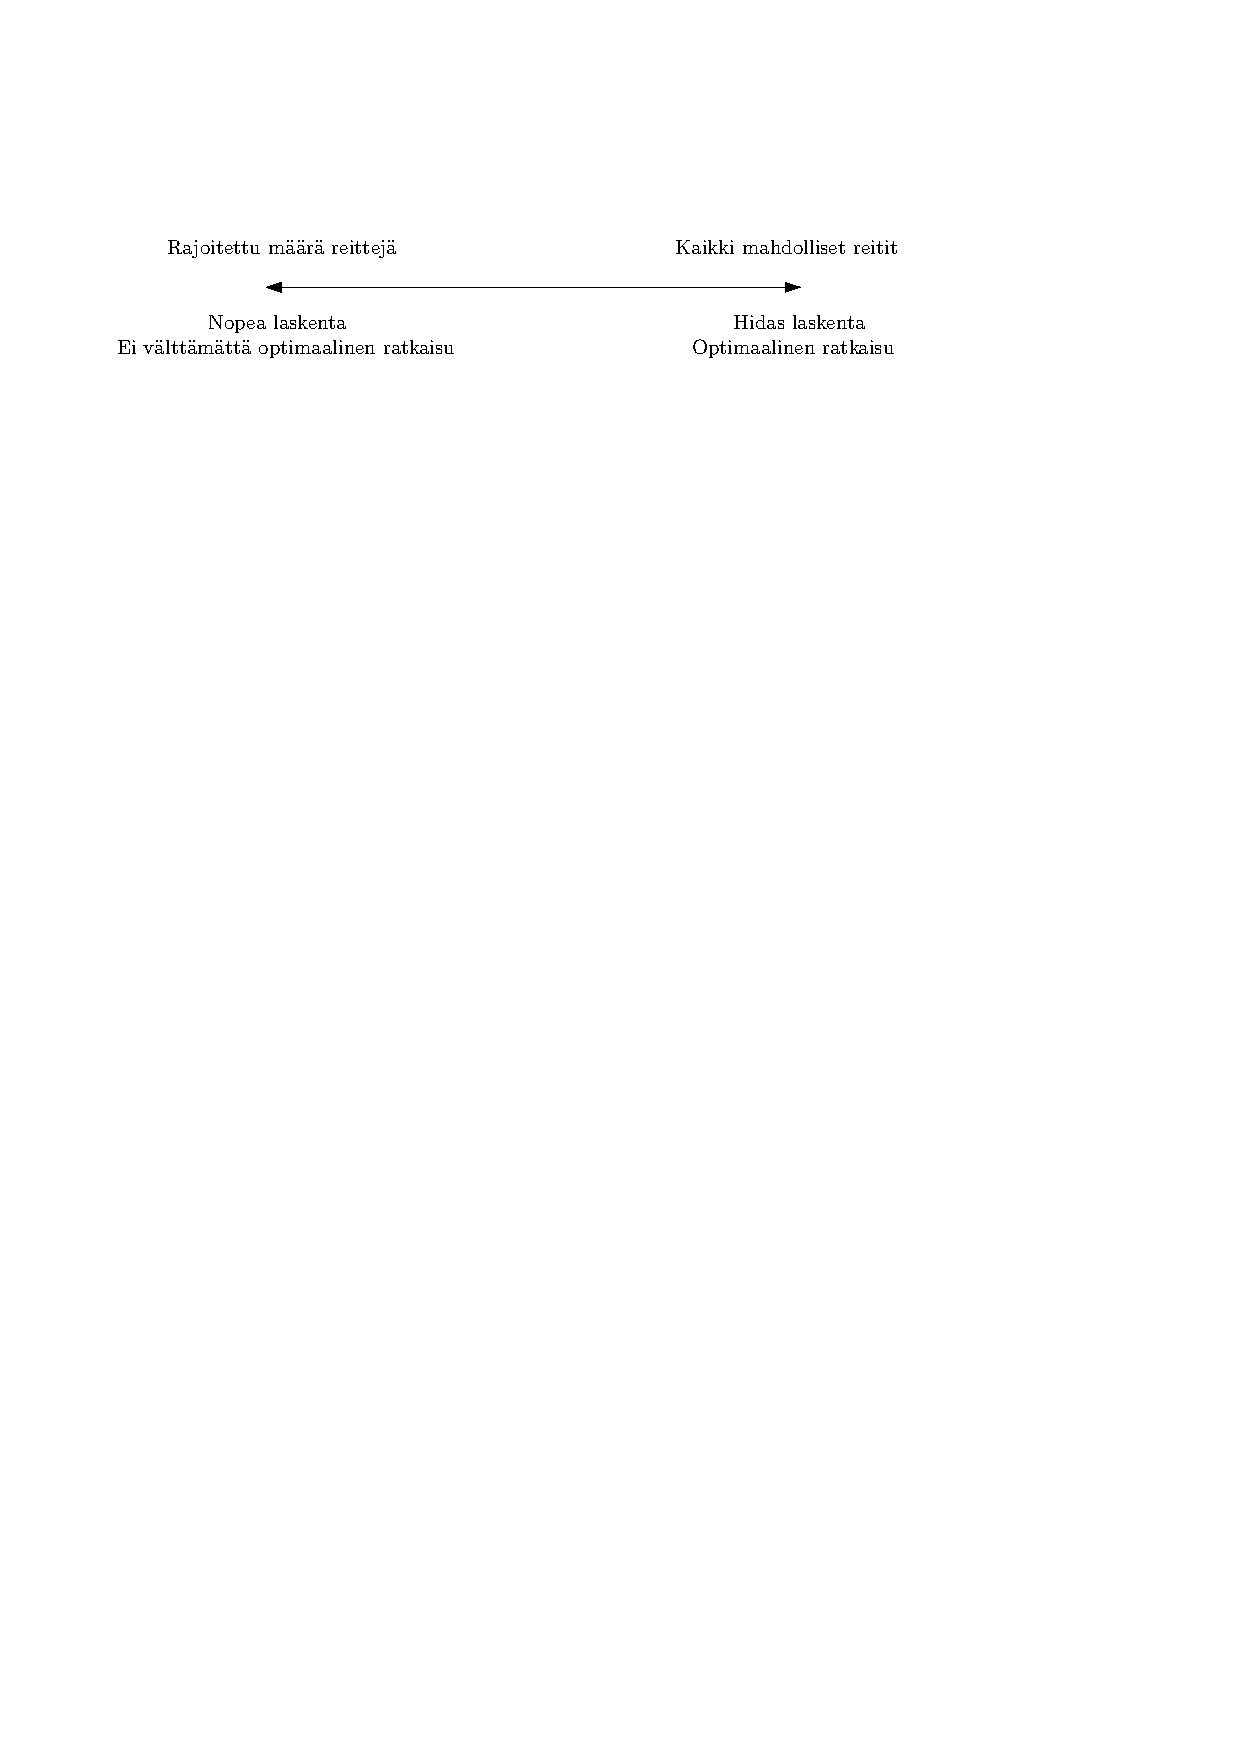
\includegraphics[scale=0.7]{vskuva}
\end{center}
\begin{itemize}
 \item 
 Yksinkertainen lisäysalgoritmi on täydellinen, kun $n < 3$
\end{itemize}

\end{frame}
    
\subsection{Keskitetty ratkaisu}
\begin{frame}
  \frametitle{Keskitetty ratkaisu}   % Insert frame title between curly braces
\begin{itemize}
\item
Uuden matkatilauksen saapuessa etsitään parasta mahdollista asiakkaiden, ajoneuvojen ja reittien yhdistelmää
\item
Toistaiseksi noutamattomien asiakkaiden ajoneuvo voi vaihtua
\item
Periaate sisältää hajautetut ratkaisut
\end{itemize}
\end{frame}

\begin{frame}
  \frametitle{Keskitetty ratkaisu, esimerkki 1} 
  \begin{minipage}{\textwidth}
    \centering
    \fbox{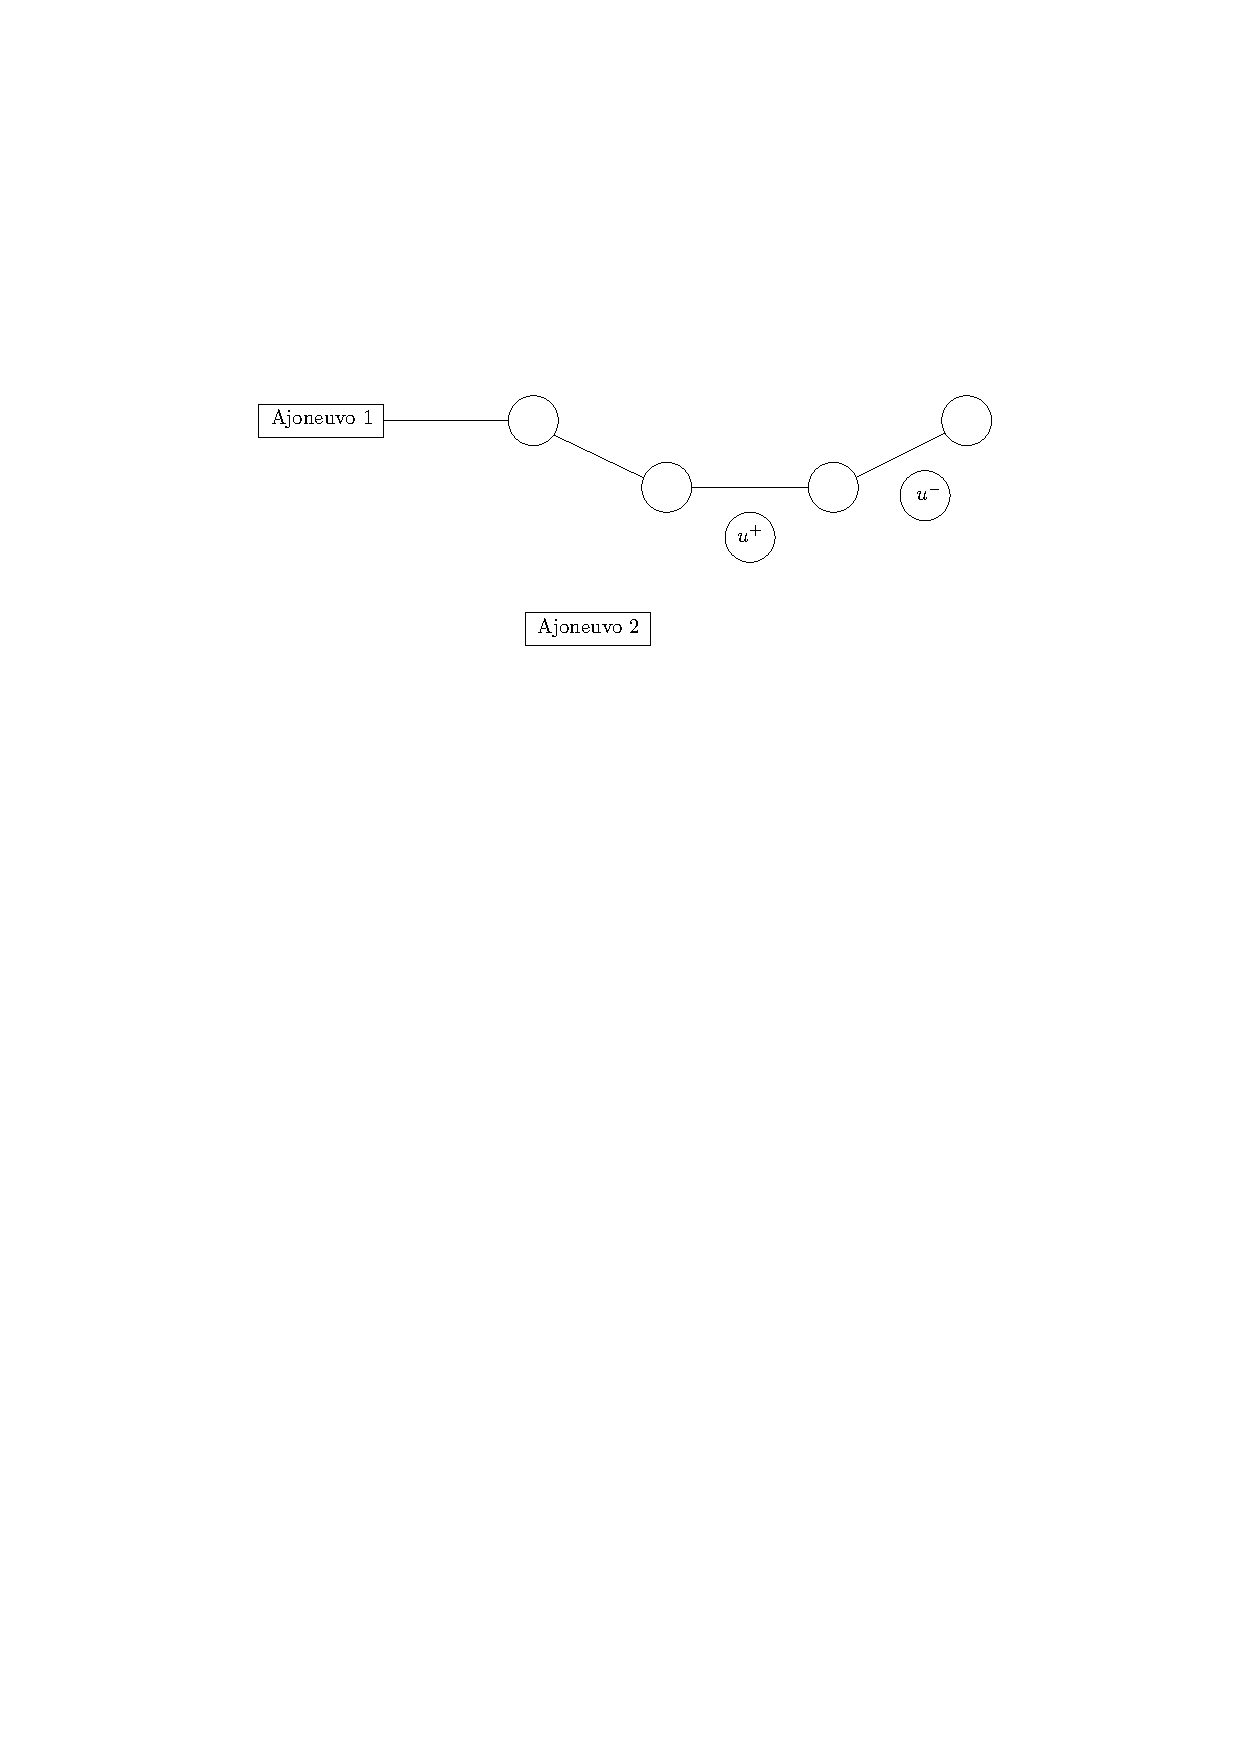
\includegraphics[scale=0.5]{valinta02}} \\
    \hfill \\
    \hfill \\
\fbox{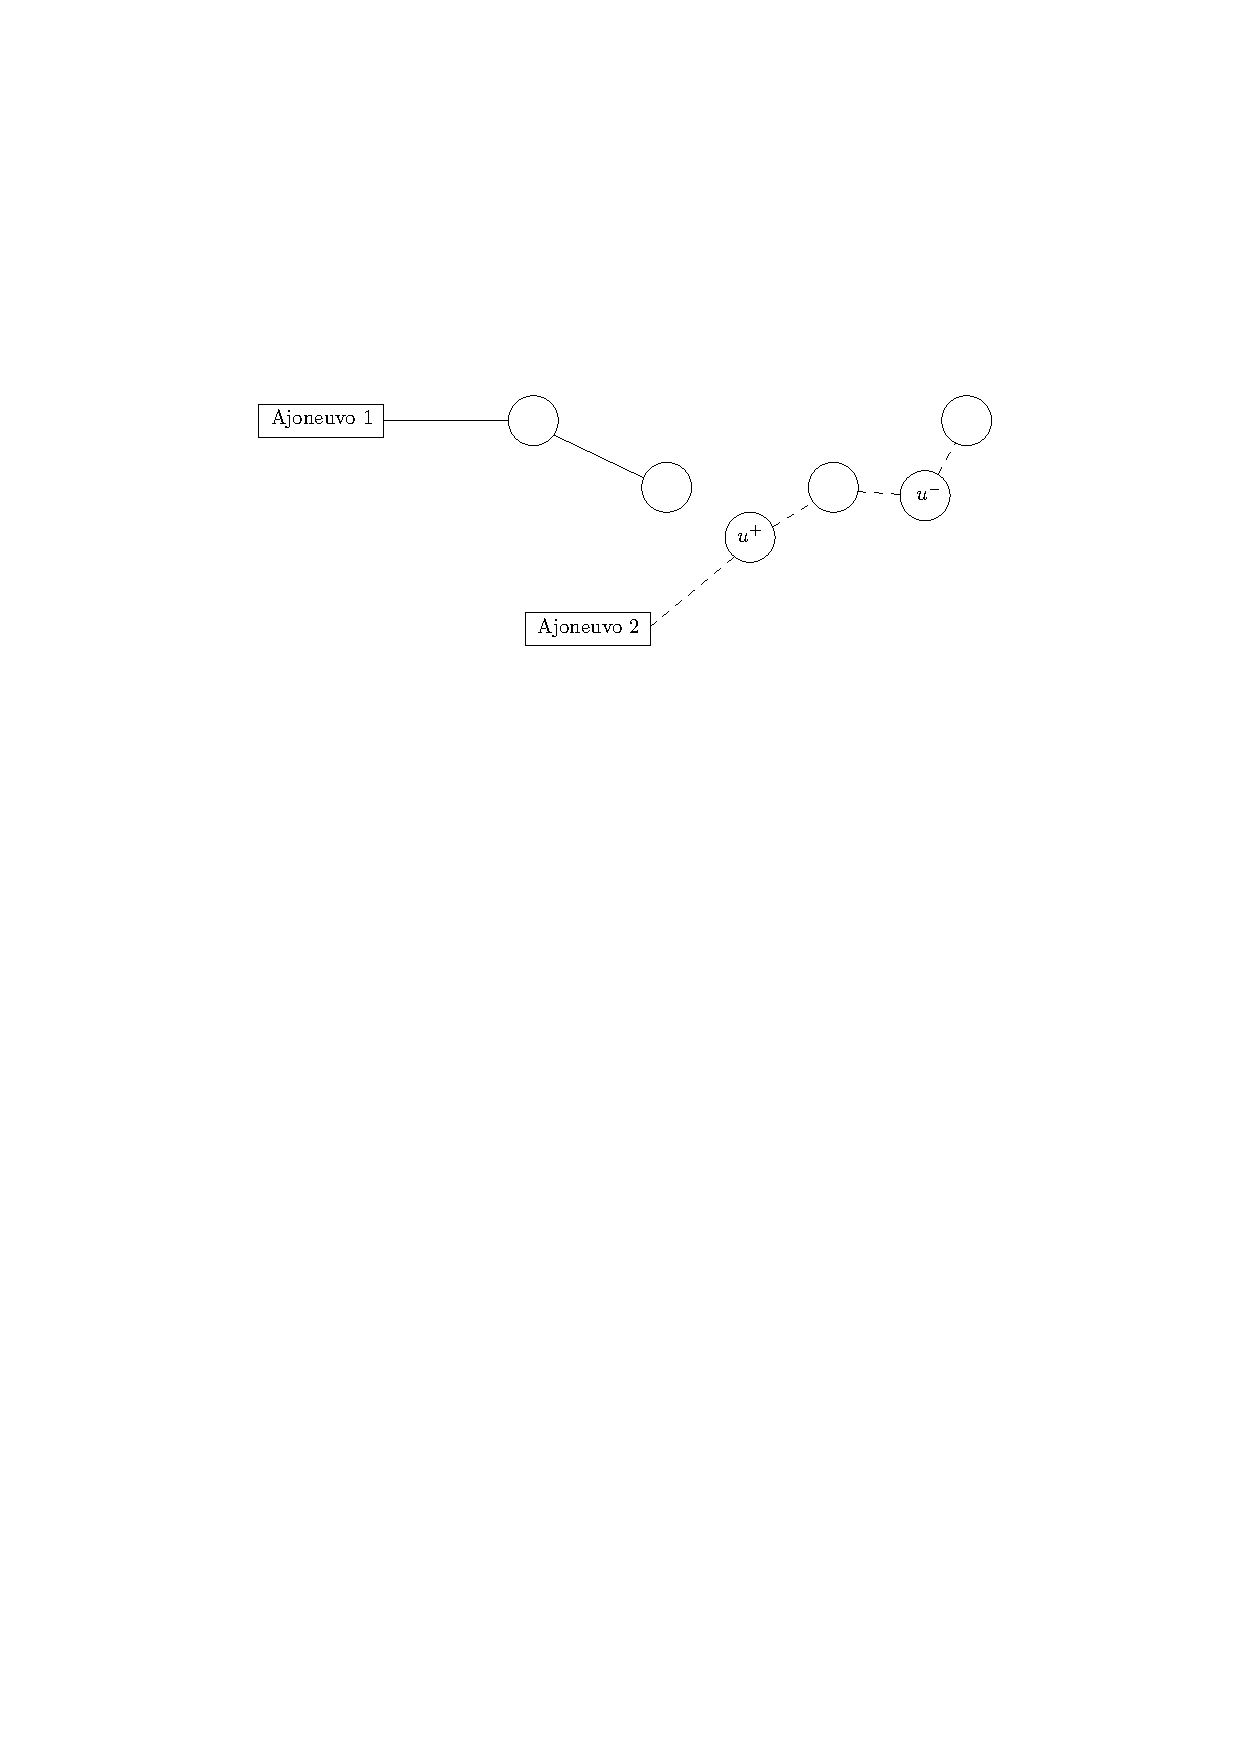
\includegraphics[scale=0.5]{valinta05}}
  \end{minipage}
\end{frame}    
    
\begin{frame}
  \frametitle{Keskitetty ratkaisu, esimerkki 2} 
  \begin{itemize}
   \item 
   Keskitetyn ratkaisun merkitys korostuu rajoitetuissa tapauksissa 
  \end{itemize}
    \begin{center}
    \includegraphics[scale=0.7]<1>{keskitettyesim01}
    \includegraphics[scale=0.7]<2>{keskitettyesim02} 
    \includegraphics[scale=0.7]<3>{keskitettyesim03} 
    \includegraphics[scale=0.7]<4>{keskitettyesim04} 
    \end{center}
\end{frame}    

\begin{frame}
  \frametitle{Maksimiklusteriperiaate (Maximum cluster algorithm)} 
  \begin{itemize}
   \item 
   Perusidea: Pyritään palvelemaan mahdollisimman suuri asiakasjoukko (klusteri) aikarajojen sisällä kullakin ajoneuvolla
   \item
   Uuden matkatilauksen saapuessa klusterit lasketaan uudelleen
  \end{itemize}
  \begin{center}
      \includegraphics[scale=0.5]<1>{maxcesim04}
      \includegraphics[scale=0.5]<2>{maxcesim03}
      \includegraphics[scale=0.5]<3>{maxcesim02}
      \includegraphics[scale=0.5]<4>{maxcesim01}
      \end{center}
\end{frame}  


\begin{frame}
  \frametitle{Arvojärjestysalgoritmi (Ranking algorithm)} 
  \begin{itemize}
   \item 
   Maksimiklusterit voidaan määrittää tehokkaasti järjestämällä nouto- ja toimituspisteet arvojärjestykseen
   \item
   Suurimman arvon saavat pisteet, joista on mahdollista siirtyä mahdollisimman moneen arvokkaaseen pisteeseen aikarajojen sisällä
   \item
   Arvojärjestys saadaan laskemalla suurinta ominaisarvoa vastaava ominaisvektori (ks. HITS-hakualgoritmi)
  \end{itemize}
  \begin{center}
      \includegraphics[scale=0.5]<1>{hub01}
      \includegraphics[scale=0.5]<2>{hub02}
      \includegraphics[scale=0.5]<3>{hub03}
      \end{center}
\end{frame}  

\begin{frame}
  \frametitle{Arvojärjestysalgoritmi, tuloksia} 
  \begin{itemize}
   \item 
    Arvojärjestysalgoritmi tuottaa tehokkaasti käypiä ratkaisuja tiukkojen rajoitusten vallitessa 
    \item
    Kertaluokkaa nopeampi aikaisempiin menetelmiin verrattuna
   \end{itemize}
\end{frame}  

% \begin{frame}
%   \frametitle{Hajautetun ja keskitetyn ratkaisun vertailu} 
%   \begin{itemize}
%    \item 
% Hajautettu ratkaisu 
% \begin{itemize}
% \item
% Laskennallisesti kevyempi
% \item
% Palvelutason kannalta luotettavampi
% \end{itemize}
% 
% \item
% Keskitetty ratkaisu
%    \begin{itemize}
% \item
% Parempi kustannustehokkuus
% \item
% Ajoneuvon vaihto ennen noutoa lisää palvelutason epävarmuutta
% \end{itemize}
%    \end{itemize}
% \end{frame}  





\section{Matkansuunnittelu}
\begin{frame}
  \frametitle{Matkansuunnittelu} 
  \begin{itemize}
   \item 
    Matkansuunnittelu (Journey planning) = joukkoliikennevälineen ja reitin valinta
    \item
    Tarkoituksena on löytää matkustajalle paras reitti ja aikataulu lähtöpisteestä määränpäähän, esim.
    \begin{itemize}
     \item 
     16:27: kävely pysäkille A,
     \item
     16:39: bussi numero 58 pysäkiltä A pysäkille B
     \item
     16:53: kävely pysäkiltä B määränpäähän, perillä klo 17:11
    \end{itemize}
   \end{itemize}
     \begin{center}
      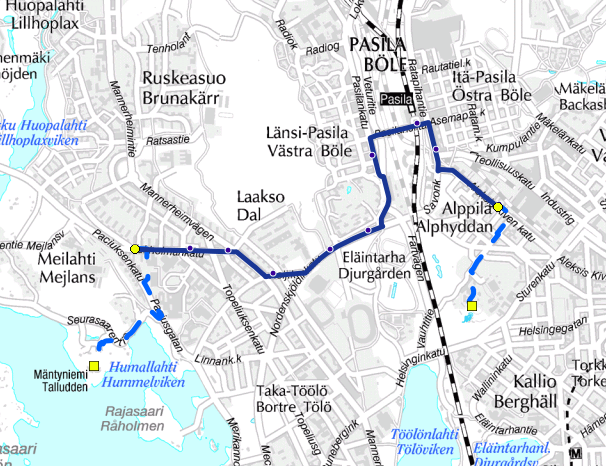
\includegraphics[scale=0.2]{reittiopas01}
      \end{center}
\end{frame} 

\begin{frame}
  \frametitle{Stokastinen malli} 
  \begin{itemize}
   \item 
    Olemassaolevilla menetelmillä voidaan laskea etukäteen paras reitti esim. matka-ajan, odotusajan, kävelymatkan tai vaihtojen lukumäärän suhteen 
    \item
    Todellisuudessa paras reitti ei välttämättä toteudu esim. myöhästymisien tai vuorojen peruutuksien takia
    \item
    Stokastinen malli ottaa huomioon mahdolliset reittimuutokset matkan varrella
    \item
    Mallin avulla voidaan laskea parhaan reitin lisäksi paras matkastrategia eri tavoitteiden suhteen
   \end{itemize}
     \begin{center}
      \end{center}
\end{frame} 

\begin{frame}
  \frametitle{Stokastinen malli, esimerkki} 
  \begin{itemize}
   \item 
    Olemassaolevilla menetelmillä voidaan laskea etukäteen paras reitti esim. matka-ajan, odotusajan, kävelymatkan tai vaihtojen lukumäärän suhteen 
    \item
    Todellisuudessa paras reitti ei välttämättä toteudu esim. myöhästymisien tai vuorojen peruutuksien takia
    \item
    Stokastinen malli ottaa huomioon mahdolliset reittimuutokset matkan varrella
    \item
    Mallin avulla voidaan laskea parhaan reitin lisäksi paras matkastrategia eri tavoitteiden suhteen
   \end{itemize}
     \begin{center}
      \end{center}
\end{frame} 

    
\end{document}